% ===========================================================================
% Eigene Abbildung (nachgebaut, KEINE fremde Grafik übernommen).
% Dreischichtiger Aufbau eines SAP-S/4HANA-Systems. Bewusst OHNE die
% positioning-Library aufgebaut (absolute Koordinaten), damit die Grafik
% unabhängig von der Präambel korrekt gestapelt kompiliert.
% Benötigt lediglich: \usepackage{tikz} in Thesis.tex.
% Ablage empfohlen: Grafiken/Kap2_Abbildung_S4HANA_Architektur.tex, per \input.
% ===========================================================================
\begin{figure}[htbp]
	\centering
	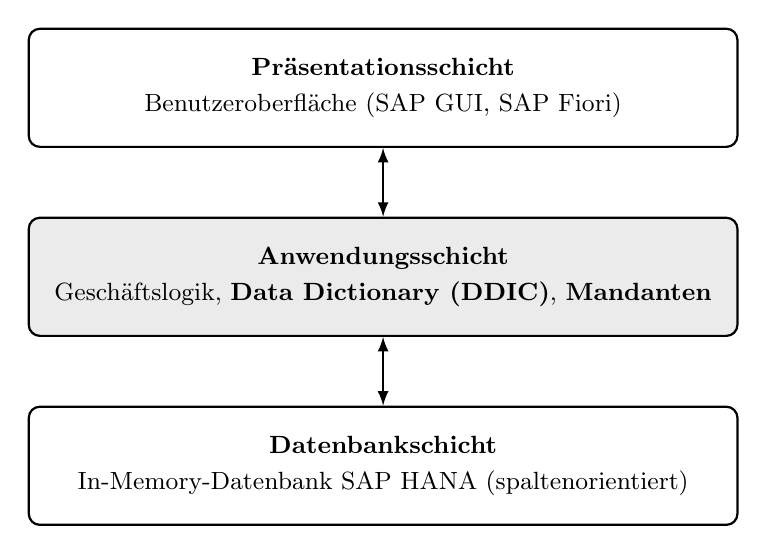
\begin{tikzpicture}[
		font=\small,
		layer/.style={draw, rounded corners, minimum width=9cm,
			minimum height=1.5cm, align=center, thick},
		hl/.style={fill=black!8},
		arr/.style={<->, >=latex, thick},
	]
		% Schichten mit absoluten Koordinaten (top-down gestapelt)
		\node[layer] (pres) at (0,0)
			{\textbf{Präsentationsschicht}\\[2pt]
			 Benutzeroberfläche (SAP GUI, SAP Fiori)};
		\node[layer, hl] (app) at (0,-2.4)
			{\textbf{Anwendungsschicht}\\[2pt]
			 Geschäftslogik, \textbf{Data Dictionary (DDIC)}, \textbf{Mandanten}};
		\node[layer] (db) at (0,-4.8)
			{\textbf{Datenbankschicht}\\[2pt]
			 In-Memory-Datenbank SAP HANA (spaltenorientiert)};

		% Verbindungen zwischen den Schichten
		\draw[arr] (pres) -- (app);
		\draw[arr] (app) -- (db);
	\end{tikzpicture}
	\caption[Dreischichtiger Aufbau eines SAP-S/4HANA-Systems]{%
		Dreischichtiger Aufbau eines SAP-S/4HANA-Systems. Die für diese Arbeit
		relevanten Elemente Data Dictionary und Mandantenfähigkeit sind in der
		Anwendungsschicht hervorgehoben. Eigene Darstellung in Anlehnung an
		Buck-Emden (1999) sowie Plattner (2009).}
	\label{fig:s4hana-architektur}
\end{figure}